\documentclass[12pt]{article}
%% arXiv paper template by Flip Tanedo
%% last updated: Dec 2016


%%%%%%%%%%%%%%%%%%%%%%%%%%%%%
%%%  THE USUAL PACKAGES  %%%%
%%%%%%%%%%%%%%%%%%%%%%%%%%%%%

\usepackage{amsmath}
\usepackage{amssymb}
\usepackage{amsfonts}
\usepackage{graphicx}
\usepackage{xcolor}
\usepackage{nopageno}
\usepackage{enumerate}
\usepackage{parskip}

%%%%%%%%%%%%%%%%%%%%%%%%%%%%%%%%%
%%%  UNUSUAL PACKAGES        %%%%
%%%  Uncomment as necessary. %%%%
%%%%%%%%%%%%%%%%%%%%%%%%%%%%%%%%%

%% MATH AND PHYSICS SYMBOLS
%% ------------------------
%\usepackage{slashed}       % \slashed{k}
%\usepackage{mathrsfs}      % Weinberg-esque letters
%\usepackage{youngtab}	    % Young Tableaux
%\usepackage{pifont}        % check marks
\usepackage{bbm}           % \mathbbm{1} incomp. w/ XeLaTeX 
%\usepackage[normalem]{ulem} % for \sout


%% CONTENT FORMAT AND DESIGN (below for general formatting)
%% --------------------------------------------------------
\usepackage{lipsum}        % block of text (formatting test)
%\usepackage{color}         % \color{...}, colored text
%\usepackage{framed}        % boxed remarks
%\usepackage{subcaption}    % subfigures; subfig depreciated
%\usepackage{paralist}      % compactitem
%\usepackage{appendix}      % subappendices
%\usepackage{cite}          % group cites (conflict: collref)
%\usepackage{tocloft}       % Table of Contents	

%% TABLES IN LaTeX
%% ---------------
%\usepackage{booktabs}      % professional tables
%\usepackage{nicefrac}      % fractions in tables,
%\usepackage{multirow}      % multirow elements in a table
%\usepackage{arydshln} 	    % dashed lines in arrays

%% Other Packages and Notes
%% ------------------------
%\usepackage[font=small]{caption} % caption font is small



\renewcommand{\thesection}{}
\renewcommand{\thesubsection}{\arabic{subsection}}

%%%%%%%%%%%%%%%%%%%%%%%%%%%%%%%%%%%%%%%%%%%%%%%
%%%  PAGE FORMATTING and (RE)NEW COMMANDS  %%%%
%%%%%%%%%%%%%%%%%%%%%%%%%%%%%%%%%%%%%%%%%%%%%%%

\usepackage[margin=2cm]{geometry}   % reasonable margins

\graphicspath{{figures/}}	        % set directory for figures

% for capitalized things
\newcommand{\acro}[1]{\textsc{\MakeLowercase{#1}}}    

\numberwithin{equation}{subsection}    % set equation numbering
\renewcommand{\tilde}{\widetilde}   % tilde over characters
\renewcommand{\vec}[1]{\mathbf{#1}} % vectors are boldface

\newcommand{\dbar}{d\mkern-6mu\mathchar'26}    % for d/2pi
\newcommand{\ket}[1]{\left|#1\right\rangle}    % <#1|
\newcommand{\bra}[1]{\left\langle#1\right|}    % |#1>
\newcommand{\Xmark}{\text{\sffamily X}}        % cross out


\let\olditemize\itemize
\renewcommand{\itemize}{
  \olditemize
  \setlength{\itemsep}{1pt}
  \setlength{\parskip}{0pt}
  \setlength{\parsep}{0pt}
}


% Commands for temporary comments
\newcommand{\comment}[2]{\textcolor{red}{[\textbf{#1} #2]}}
\newcommand{\flip}[1]{{\color{red} [\textbf{Flip}: {#1}]}}
\newcommand{\email}[1]{\texttt{\href{mailto:#1}{#1}}}

\newenvironment{institutions}[1][2em]{\begin{list}{}{\setlength\leftmargin{#1}\setlength\rightmargin{#1}}\item[]}{\end{list}}


\usepackage{fancyhdr}		% to put preprint number



%%%%%%%%%%%%%%%%%%%
%%%  HYPERREF  %%%%
%%%%%%%%%%%%%%%%%%%

%% This package has to be at the end; can lead to conflicts
\usepackage{microtype}
\usepackage[
	colorlinks=true,
	citecolor=black,
	linkcolor=black,
	urlcolor=green!50!black,
	hypertexnames=false]{hyperref}



%%%%%%%%%%%%%%%%%%%%%
%%%  TITLE DATA  %%%%
%%%%%%%%%%%%%%%%%%%%%

\begin{document}


\begin{center}

    {\Large \textsc{Homework 3a:} 
    \textbf{Analytic functions are \emph{too} nice}}
    
\end{center}

\vskip .4cm

\noindent
\begin{tabular*}{\textwidth}{rlcrll}
	\textsc{Course:}& Physics 231, \emph{Methods of Theoretical Physics} (2018)
	&
%	\hspace{1.2cm}
	&
	\\
	\textsc{Instructor:}& Professor Flip Tanedo (\email{flip.tanedo@ucr.edu})
	&
	%\hfill
	&
	& 
	\\
	\textsc{Due by:}& Wed, October 31
	&
	%\hfill
	&
	%	
\end{tabular*}

\textbf{Cauchy's Integral Formula} is the powerful statement that the integral of an analytic function, $f(z)$ over any closed loop $C$, is zero:
\begin{align}
	\oint_C dz\; f(z) = 0 \ .
	\label{eq:cauchy}
\end{align}
In other words, analytic functions are not only nice, they are \emph{too nice}---their integrals don't contain any information!
%
In this mini-homework we prove  the integral formula in two ways: a \emph{little tiny} circle and a \emph{little tiny} square.
%



\subsection{Little tiny circle} 

We show that the Cauchy integral formula (\ref{eq:cauchy}) holds for the a small, counter-clockwise circular path of radius $\epsilon$ around the point $z_0$:
\begin{center}
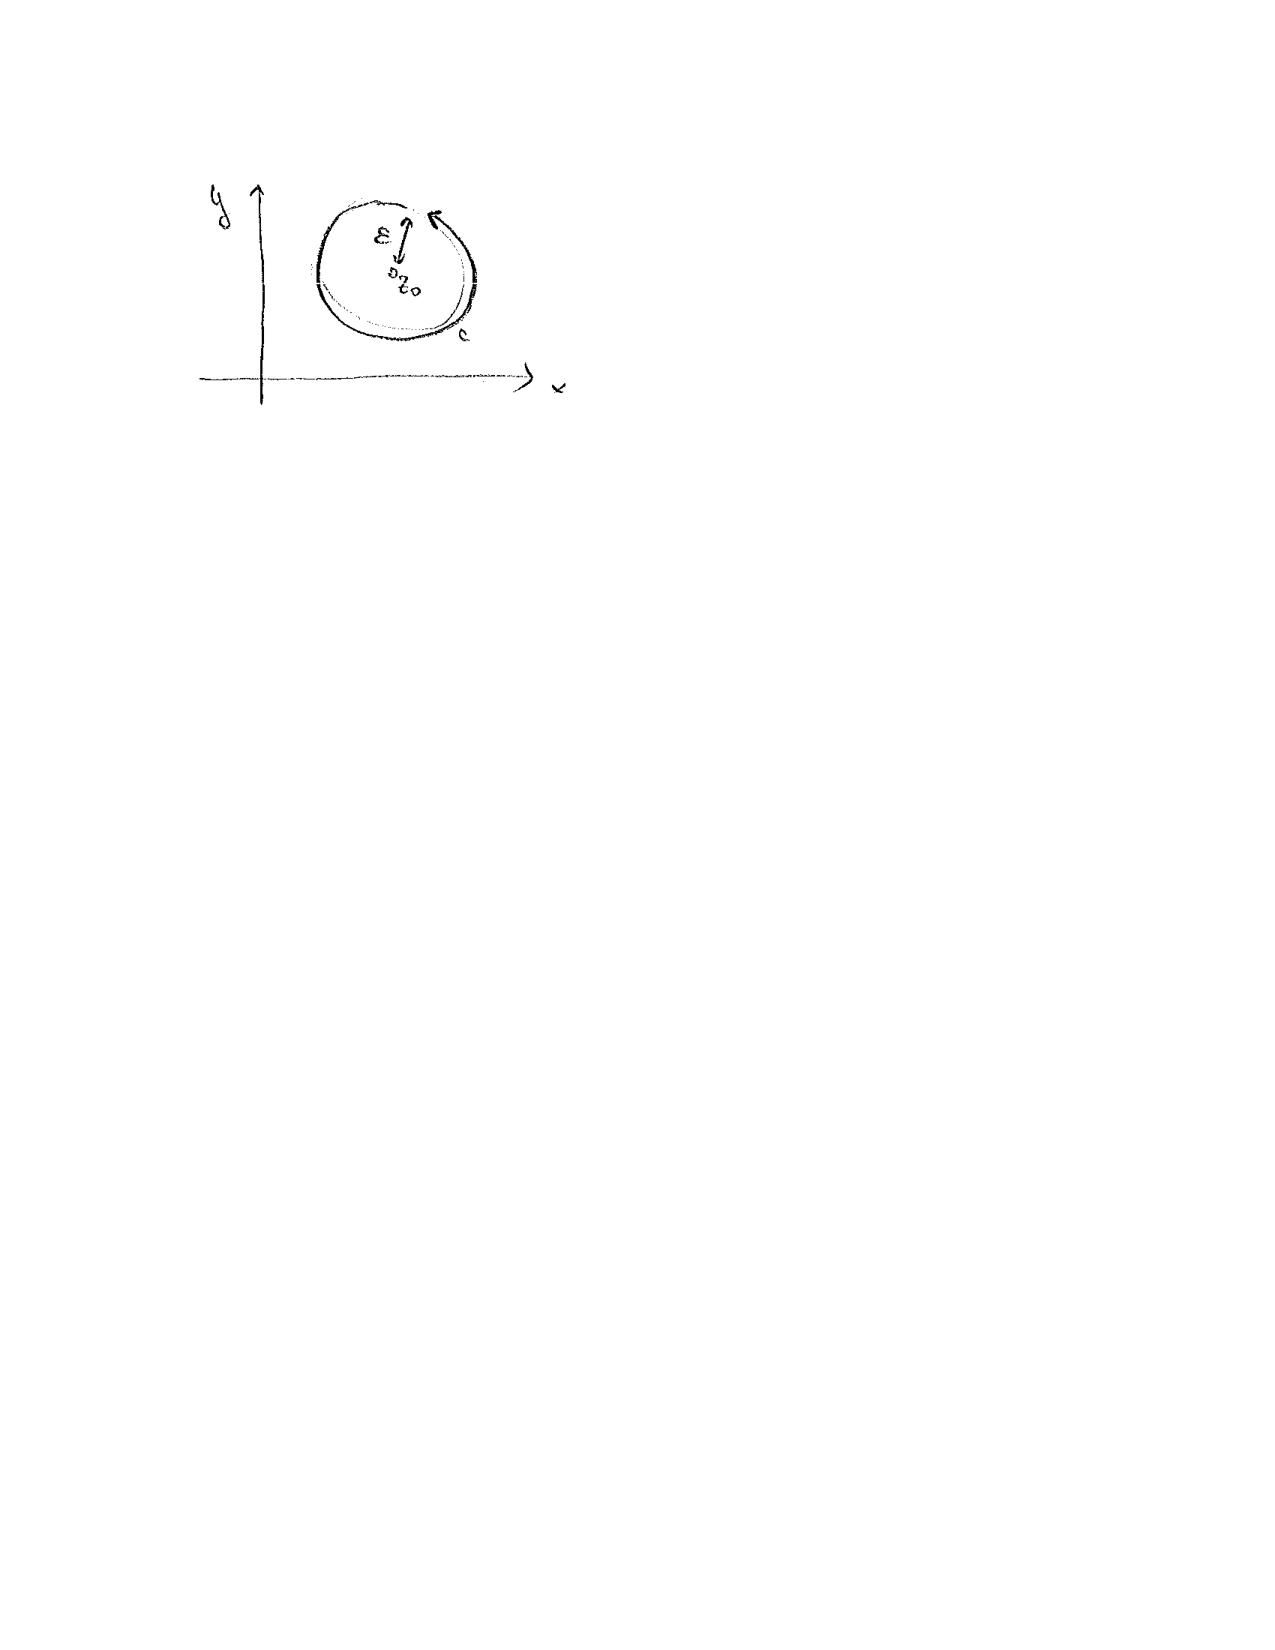
\includegraphics[width=.3\textwidth]{P231_2018_HW3a_fig1}
\end{center}

\subsubsection{Parameterize the path}

Parameterize the path in terms of the polar angle $\theta$:
\begin{align}
	z(\theta) = z_0 + \epsilon e^{i\theta} \ .
\end{align}
Write the left-hand side of (\ref{eq:cauchy}) as a definite integral by filling in the right-hand side of the following:
\begin{align}
	\oint_C dz\; f(z)
	&= 
	\int_0^{2\pi} d\theta \;
	f\left(z(\theta)\right) (\cdots) \ .
\end{align}
Fill in the facotr $``\cdots''$.

\subsubsection{Leading terms}

Taylor expand $f(z)$ about $z = z_0$. Keep the zeroth and first order terms and plug them into the $d\theta$ integral. Write the two terms in the integrand as explicit functions of $\epsilon$ and $\theta$:
\begin{align}
	\oint_C dz\; f(z) 
	& = 
	\int_0^{2\pi} d\theta \; \left[ \text{ function of only }\epsilon\text{ and }\theta\text{ } \right]
\end{align}

\subsubsection{Argue that the integral vanishes}

Argue that the $d\theta$ integral indeed vanishes. Did you have to use $\epsilon \to 0$?

\subsection{Little tiny square(s)}

Now show that the Cauchy integral formula (\ref{eq:cauchy}) holds for the a small, counter-clockwise square path of length $\epsilon$ around the point $z_0$:
\begin{center}
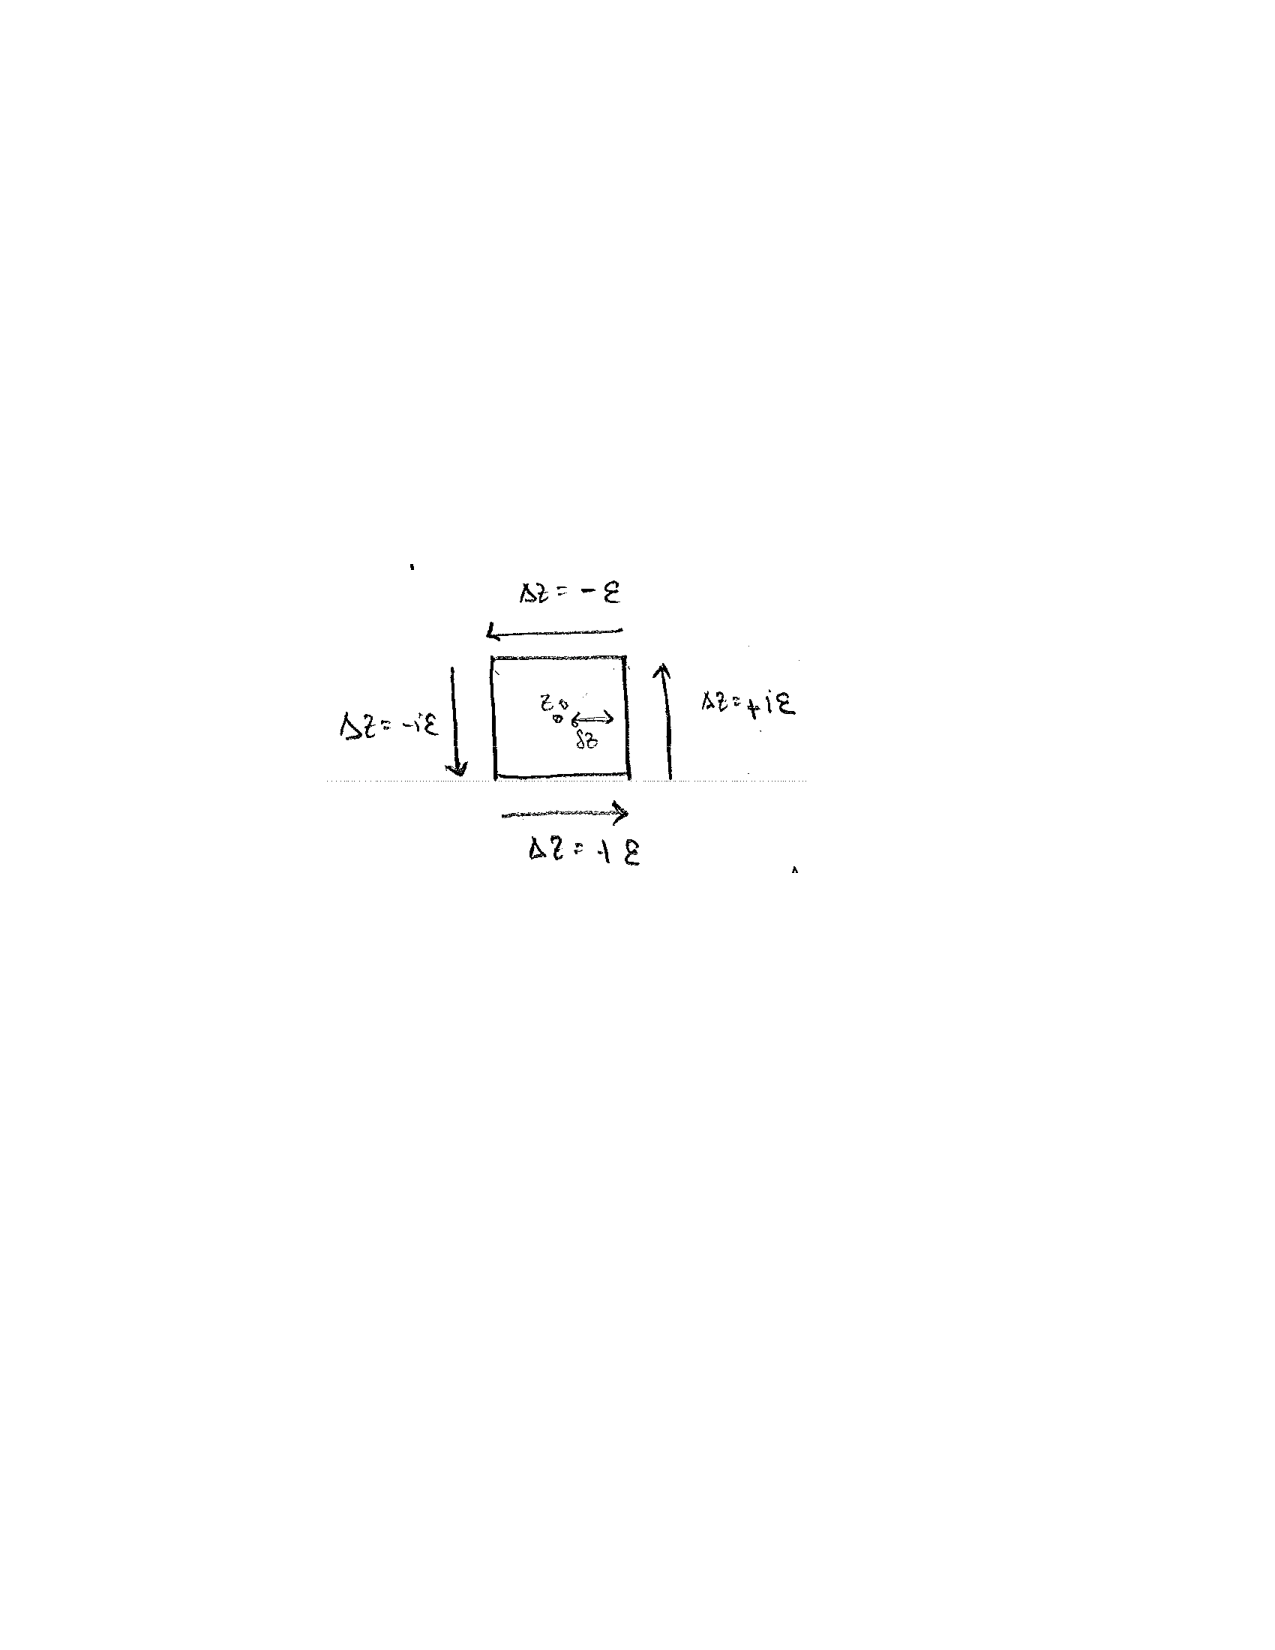
\includegraphics[width=.3\textwidth]{P231_2018_HW3a_fig2}
\end{center}

\subsubsection{Parameterize the path, leading terms}

Decompose the path into four straight line pieces, $\Delta z_1$, $\cdots$, $\Delta z_4$. For each leg, do a Taylor expansion and keep the zeroth and first order terms. Write the integral as
\begin{align}
	\oint_C dz\; f(z) &=
	f(z_0) \left[ \cdots \right]
	+ f'(z_0) \left[ \cdots \right] \ ,
\end{align}
	where you fill in the ``$\cdots$''. 

\subsubsection{Argue that the integral vanishes}

Show that both of the ``$\cdots$'' terms vanish. \textsc{Hint}: it may be useful to think of $dz = \Delta z$ in the integral and $(z-z_0) = \delta z$ in the Taylor expansion as two separate quantities that depend on $\epsilon$.


\subsection{Where did we use analyticity?}

Why don't these proofs hold for \emph{any} complex function? Where did we use the fact that the function $f(z)$ is \emph{analytic}? 
\textsc{Hint}: it was important that our contours were ``little tiny'' shapes. 




\section{Extra Credit}

These problems are not graded and are for your edification. You are strongly encouraged to explore and discuss these topics, especially if they are in a field of interest to you.

\subsection{Cauchy Integral Theorem And Conservative Forces} 

I made an incorrect statement in response to a question from Christopher two weeks ago. The Cauchy integral theorem \emph{is} related to conservative forces. Using whatever resources you wish (I suggest starting with Google), describe the nature of this relation.


\subsection{Spot the error} 

What's wrong with the following sequence of steps:
\begin{align}
	e^{2\pi i} &= 1 \\
	\left(e^{2\pi i}\right)^{2\pi i} &= 1^{2\pi i} = 1 \\
	\left(e^{-2\pi}\right)^2 &= 1   \\ 
	e^{-4\pi} &= 1 \ .
\end{align}
But since $e^x =1 \Rightarrow x = 0$, this means that $\pi = 0$. 


\end{document}